% ============================================================
%  main.tex  –  Converted from input.docx
%  To compile: pdflatex main.tex  (run twice for references)
% ============================================================
\documentclass[12pt, a4paper]{article}

% ---------- Encoding & fonts ----------
\usepackage[T1]{fontenc}
\usepackage[utf8]{inputenc}
\usepackage{lmodern}
\usepackage{microtype}

% ---------- Page layout ----------
\usepackage[margin=1in]{geometry}

% ---------- Colours ----------
\usepackage{xcolor}

% ---------- Tables ----------
\usepackage{longtable, booktabs, array}
\usepackage{calc}
\usepackage{etoolbox}
\makeatletter
\patchcmd\longtable{\par}{\if@noskipsec\mbox{}\fi\par}{}{}
\makeatother
\IfFileExists{footnotehyper.sty}{\usepackage{footnotehyper}}{\usepackage{footnote}}
\makesavenoteenv{longtable}

% ---------- Graphics ----------
\usepackage{graphicx}
\graphicspath{{figures/}}          % <-- all images live in figures/
\makeatletter
\def\maxwidth{\ifdim\Gin@nat@width>\linewidth\linewidth\else\Gin@nat@width\fi}
\def\maxheight{\ifdim\Gin@nat@height>0.6\textheight 0.6\textheight\else\Gin@nat@height\fi}
\makeatother
\setkeys{Gin}{width=\maxwidth, height=\maxheight, keepaspectratio}

% ---------- Hyperlinks ----------
\usepackage[hidelinks]{hyperref}
\usepackage{xurl}
\urlstyle{same}

% ---------- Misc ----------
\setlength{\emergencystretch}{3em}
\providecommand{\tightlist}{%
  \setlength{\itemsep}{0pt}\setlength{\parskip}{0pt}}
\setcounter{secnumdepth}{-\maxdimen}   % no section numbers (matches original)

% ============================================================
\begin{document}

% ----------------------------------------------------------------
\section*{Appendix A -- Enhanced Use Case Diagram}
% ----------------------------------------------------------------

The enhanced use case diagram consolidates the original 9 PS use cases
(UC-01 through UC-09) into 5 high-level user goals as defined during the
Analysing phase:

\begin{itemize}
  \item \textbf{UC-1: Identify Music in the Moment} -- Encompasses PS UC-01
        (Discover Music) and UC-06 (Provide Consent).
  \item \textbf{UC-2: Understand a Song and Decide Next Action} -- Encompasses
        PS UC-03 (View Music Information) and UC-07 (View Similar Music).
  \item \textbf{UC-3: Continue Listening via Official Sources} -- Encompasses
        PS UC-05 (Open Streaming Platform).
  \item \textbf{UC-4: Build a Personal Music Library} -- Encompasses PS UC-04
        (Save/View History), UC-08 (Add to Favourites), UC-09 (View Favourites).
  \item \textbf{UC-5: Control Data and Permissions} -- Encompasses privacy
        consent, microphone permissions, and data management settings.
\end{itemize}

\begin{figure}[htbp]
  \centering
  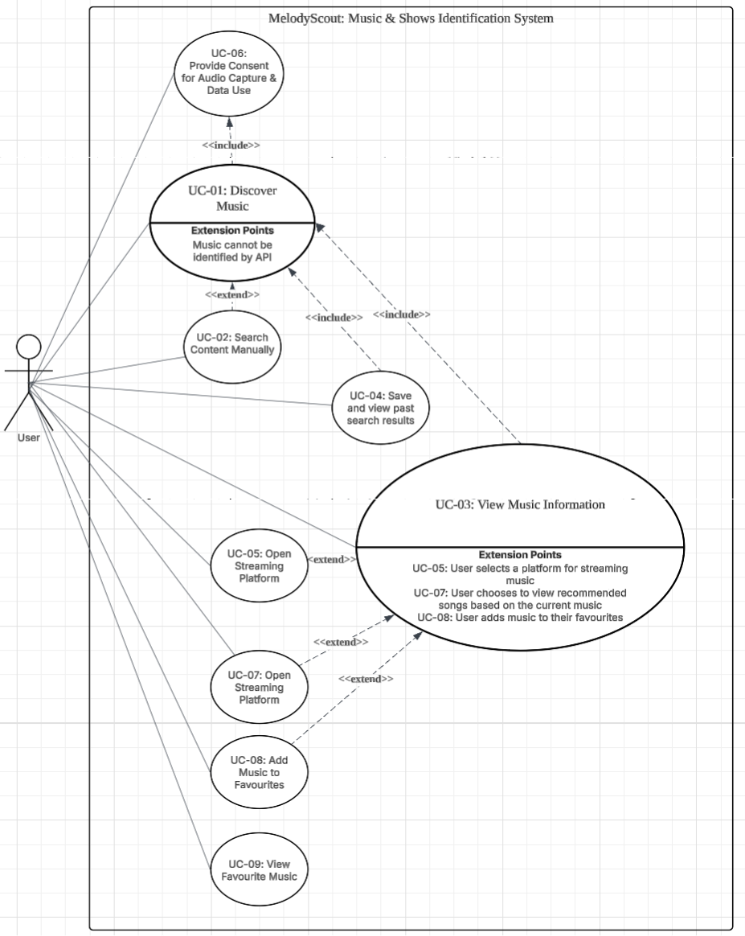
\includegraphics[width=0.75\linewidth]{figure1}
  \caption{Enhanced Use Case Diagram}
\end{figure}

% ----------------------------------------------------------------
\section*{Appendix B -- Refined Data Dictionary}
% ----------------------------------------------------------------

The refined data dictionary includes all original PS entities with
vendor-proposed enhancements from the Analysing Report. The following
tables are documented with full attribute definitions:

\textbf{Original PS Tables (maintained):} User, UserConsent,
ContentMetadata, AudioIdentification, SearchHistory, UserFavorites,
StreamingPlatform, ContentAvailability, APIConfiguration, AppSettings.

\textbf{Enhanced Attributes:} User table -- \texttt{subscription\_tier}
(\texttt{FREE|PREMIUM}), \texttt{preferred\_language}
(\texttt{EN|ZH|MS|TA}), \texttt{notification\_consent} (\texttt{BOOLEAN});
AudioIdentification table -- \texttt{deletion\_timestamp} (\texttt{DATETIME}),
\texttt{network\_type} (\texttt{3G|4G|5G|WIFI}), \texttt{error\_code}
(\texttt{VARCHAR}).

\textbf{New Tables:} \texttt{APIUsageTracking} (\texttt{usage\_id},
\texttt{api\_service}, \texttt{request\_timestamp},
\texttt{response\_time\_ms}, \texttt{status\_code},
\texttt{monthly\_cumulative\_count}); \texttt{CrossDeviceSyncLog}
(\texttt{sync\_id}, \texttt{user\_id}, \texttt{device\_id},
\texttt{sync\_type}, \texttt{sync\_timestamp}, \texttt{sync\_status}).

\textbf{Repository Location:}
\url{https://github.com/TechForge/beatfinder-requirements-repo/tree/main/data-dictionary/}

% ----------------------------------------------------------------
\section*{Appendix C -- Wireframes}
% ----------------------------------------------------------------

Mobile application wireframes are carried forward from PS Section~8.3
depicting the following screens: Home Screen (Identify Song CTA),
Listening Animation, Song Result (with Add to Favourites, View Similar
Songs, streaming platform deep links), History View (searchable),
Favourites View, Settings Screen (Microphone Access, Clear History,
Privacy Policy, Terms of Service), Recommendations Screen (Songs Similar
To), and Manual Search Fallback screens (audio failure and text input).

\begin{figure}[htbp]
  \centering
  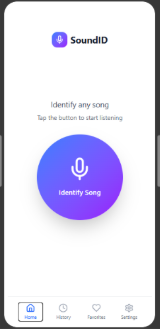
\includegraphics[height=5cm]{figure2}\hspace{2pt}%
  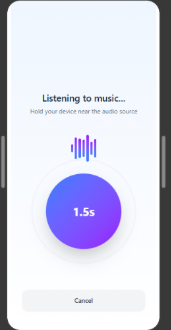
\includegraphics[height=5cm]{figure3}\hspace{2pt}%
  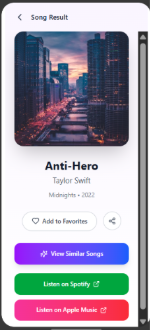
\includegraphics[height=5cm]{figure4}\hspace{2pt}%
  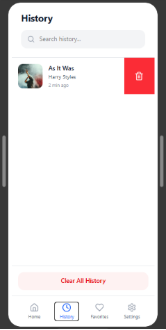
\includegraphics[height=5cm]{figure5}\hspace{2pt}%
  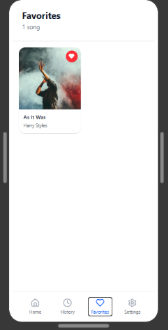
\includegraphics[height=5cm]{figure6}\hspace{2pt}%
  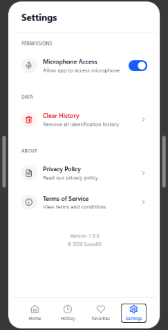
\includegraphics[height=5cm]{figure7}\hspace{2pt}%
  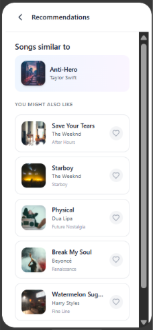
\includegraphics[height=5cm]{figure8}\\[4pt]
  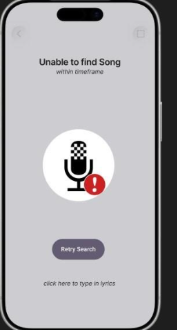
\includegraphics[height=5cm]{figure9}\hspace{2pt}%
  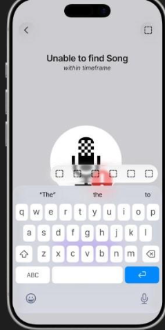
\includegraphics[height=5cm]{figure10}
  \caption{Mobile Application Wireframes}
\end{figure}

\textbf{Repository Location:}
\url{https://github.com/ssimplee/ICT2113_P2-3010A}

% ----------------------------------------------------------------
\section*{Appendix D -- Prototype}
% ----------------------------------------------------------------

\begin{figure}[htbp]
  \centering
  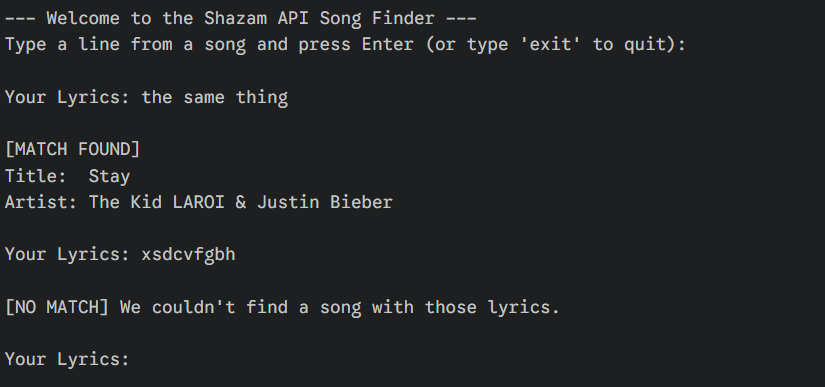
\includegraphics[width=\linewidth]{figure11}
  \caption{Prototype Overview}
\end{figure}

\textbf{Repository Location:}
\url{https://github.com/ssimplee/ICT2113_P2-3010A}

% ----------------------------------------------------------------
\section*{Appendix E -- Internal Requirements Traceability Matrix (iRTM)}
% ----------------------------------------------------------------

\subsection*{Functional Requirements Traceability}

\begin{longtable}[]{@{}
  >{\raggedright\arraybackslash}p{0.15\linewidth}
  >{\raggedright\arraybackslash}p{0.12\linewidth}
  >{\raggedright\arraybackslash}p{0.18\linewidth}
  >{\raggedright\arraybackslash}p{0.38\linewidth}
  >{\raggedright\arraybackslash}p{0.10\linewidth}@{}}
\toprule
\textbf{RTM ID} & \textbf{Source} & \textbf{SRS Req} &
\textbf{Description} & \textbf{Method} \\
\midrule
\endhead
\bottomrule
\endlastfoot
\textbf{SRS-RTM-001} & PS UC-01 & SRS-FR-AUD-001 & Audio-based music identification via microphone capture & Duplicate \\
\textbf{SRS-RTM-002} & PS UC-02 & SRS-FR-SRCH-001 & Manual text search when auto-identification unavailable & Duplicate \\
\textbf{SRS-RTM-003} & PS UC-03 & SRS-FR-META-001 & Display song metadata (title, artist, album, genre) & Paraphrase \\
\textbf{SRS-RTM-004} & PS UC-04 & SRS-FR-LIB-002 & Save and view past search results in history & Duplicate \\
\textbf{SRS-RTM-005} & PS UC-05 & SRS-FR-STR-001 & Open external streaming platform for content & Minimized \\
\textbf{SRS-RTM-006} & PS UC-06 & SRS-NFR-PRIV-001 & Consent for audio capture and data use before first use & Paraphrase \\
\textbf{SRS-RTM-007} & PS UC-07 & SRS-FR-REC-004 & View similar/recommended music & Minimized \\
\textbf{SRS-RTM-008} & PS UC-08 & SRS-FR-LIB-001 & Add music to personal favourites & Duplicate \\
\textbf{SRS-RTM-009} & PS UC-09 & SRS-FR-LIB-003 & View favourite music collection & Duplicate \\
\end{longtable}

\subsection*{Business \& Technical Requirements Traceability}

\begin{longtable}[]{@{}
  >{\raggedright\arraybackslash}p{0.15\linewidth}
  >{\raggedright\arraybackslash}p{0.12\linewidth}
  >{\raggedright\arraybackslash}p{0.18\linewidth}
  >{\raggedright\arraybackslash}p{0.38\linewidth}
  >{\raggedright\arraybackslash}p{0.10\linewidth}@{}}
\toprule
\textbf{RTM ID} & \textbf{Source} & \textbf{SRS Req} &
\textbf{Description} & \textbf{Method} \\
\midrule
\endhead
\bottomrule
\endlastfoot
\textbf{SRS-RTM-010} & PS CNST-001 & SRS-NFR-UX-001 & CineBeat brand identity integration (\#FF5722, \#1A1A1A) & Duplicate \\
\textbf{SRS-RTM-011} & PS CNST-002 & SRS-FR-AUD-004 & Audio deletion post-processing (revised to 3s per CLAR-001) & Paraphrase \\
\textbf{SRS-RTM-012} & PS CNST-003 & SRS-FR-EDT-001 & Redirect to CineBeat website for full reviews & Duplicate \\
\textbf{SRS-RTM-013} & PS CNST-004 & IMPL-001 & Waterfall SDLC methodology compliance & Duplicate \\
\textbf{SRS-RTM-014} & PS REQ-TECH-001 & SRS-TPR-MOB-001 & Cross-platform mobile framework (single codebase) & Duplicate \\
\textbf{SRS-RTM-015} & PS REQ-TECH-004 & SRS-TPR-DB-002 & Azure SQL Database (revised from Data Studio per CLAR-002) & Paraphrase \\
\textbf{SRS-RTM-016} & PS REQ-TECH-005 & SRS-TPR-API-001 & Shazam API v1 via RapidAPI integration & Duplicate \\
\textbf{SRS-RTM-017} & PS REQ-TECH-006 & SRS-TPR-NET-001 & HTTPS with TLS 1.3 security & Duplicate \\
\textbf{SRS-RTM-018} & AR CLAR-003 & SRS-FR-REC-001 & Spotify API + collaborative filtering for recommendations & Paraphrase \\
\textbf{SRS-RTM-019} & AR CLAR-005 & SRS-TPR-API-004 & API rate limiting and throttling strategy (100K/month) & Paraphrase \\
\textbf{SRS-RTM-020} & AR CLAR-006 & SRS-FR-SYNC-001 & Cross-device sync for favourites and history only & Minimized \\
\textbf{SRS-RTM-021} & PS REG-001 & SRS-NFR-PRIV-001 & PDPA compliance for user consent and data collection & Duplicate \\
\textbf{SRS-RTM-022} & PS REG-002 & SRS-NFR-PRIV-002 & GDPR compliance for data portability and right to be forgotten & Paraphrase \\
\end{longtable}

\subsection*{Quality \& Change Traceability}

\begin{longtable}[]{@{}
  >{\raggedright\arraybackslash}p{0.15\linewidth}
  >{\raggedright\arraybackslash}p{0.12\linewidth}
  >{\raggedright\arraybackslash}p{0.18\linewidth}
  >{\raggedright\arraybackslash}p{0.38\linewidth}
  >{\raggedright\arraybackslash}p{0.10\linewidth}@{}}
\toprule
\textbf{RTM ID} & \textbf{Source} & \textbf{SRS Req} &
\textbf{Description} & \textbf{Method} \\
\midrule
\endhead
\bottomrule
\endlastfoot
\textbf{SRS-RTM-023} & SRS-QDM-AFA & SRS-FR-AUD-003 & Acoustic Fidelity: 5s identification SLA & Paraphrase \\
\textbf{SRS-RTM-024} & SRS-QDM-ERI & SRS-FR-EDT-001 & Ecosystem Retention: editorial content bridge & Minimized \\
\textbf{SRS-RTM-025} & SRS-QDM-PCI & SRS-NFR-PRIV-005 & Privacy Compliance: deletion audit trail & Paraphrase \\
\textbf{SRS-RTM-026} & SRS-QDM-CPBP & SRS-TPR-MOB-001 & Cross-Platform Parity: single codebase & Minimized \\
\textbf{SRS-RTM-027} & SRS-QDM-ARG & SRS-TPR-API-004 & Resource Governance: API throttling strategy & Paraphrase \\
\end{longtable}

\end{document}
